\section{Метод конечных разностей во временной области}

Для расчетов спектра пропускания и локального распределения плотности мощности электромагнитного поля димеров плазмонных наночастиц часто используют метод конечных разностей во временной области. Метод конечных разностей во временной области (англ. Finite Difference Time Domain, FDTD) — один из наиболее популярных методов численной электродинамики, основанный на дискретизации уравнений Максвелла, записанных в дифференциальной форме. Рассмотрим базовый алгоритм Йи для численного решения уравнений Максвелла, первоначально использованный в методе FDTD и подробно изложенный в статье~\cite{FDTDYee}.

Уравнения Максвелла в изотропной среде в системе СИ имеют вид:
\begin{subequations}
\begin{gather}
\dfrac{\partial \textbf{B}}{\partial t} + \nabla \times \textbf{E} = 0, \label{eq:MaxwellA} \\
- \dfrac{\partial \textbf{D}}{\partial t} + \nabla \times \textbf{H} = \textbf{J}, \label{eq:MaxwellB} \\
\nabla \cdot \textbf{D} = \rho \label{eq:MaxwellC}, \\
\nabla \cdot \textbf{B} = 0 \label{eq:MaxwellD}.
\end{gather}
\end{subequations}

В декартовых координатах уравнения~(\ref{eq:MaxwellA}) и~(\ref{eq:MaxwellB}) эквивалентны следующей системе скалярных уравнений:

\begin{subequations}
\begin{gather}
- \dfrac{\partial B_x}{\partial t} = \dfrac{\partial E_z}{\partial y} - \dfrac{\partial E_y}{\partial z} \label{eq:scalarMEa}, \\
- \dfrac{\partial B_y}{\partial t} = \dfrac{\partial E_x}{\partial z} - \dfrac{\partial E_z}{\partial x} \label{eq:scalarMEb}, \\
\dfrac{\partial B_z}{\partial t} = \dfrac{\partial E_x}{\partial y} - \dfrac{\partial E_y}{\partial x} \label{eq:scalarMEc}, \\
- \dfrac{\partial D_x}{\partial t} = \dfrac{\partial H_z}{\partial y} - \dfrac{\partial H_y}{\partial z}+J_x \label{eq:scalarMEd}, \\
- \dfrac{\partial D_y}{\partial t} = \dfrac{\partial H_x}{\partial z} - \dfrac{\partial H_z}{\partial x}+J_y \label{eq:scalarMEe}, \\
- \dfrac{\partial D_z}{\partial t} = \dfrac{\partial H_y}{\partial x} - \dfrac{\partial H_x}{\partial y}+J_z \label{eq:scalarMEf}.
\end{gather}
\end{subequations}
Вводя разностную сетку, для точки в пространстве получим:
\begin{equation}
(i, j, k) = (i \Delta x, j \Delta y, k \Delta z),
\label{eq:pointgrid}
\end{equation}
и для любой функции координат и времени положим:
\begin{equation}
F(i \Delta x, j \Delta y, k \Delta z, n \Delta t ) = F^n (i, j, k).
\label{eq:funcgrid}
\end{equation}

При идеально проводящих граничных условиях система разностных уравнений~(\ref{eq:scalarMEa})~--~(\ref{eq:scalarMEf}) выглядит следующим образом. Для~(\ref{eq:scalarMEa}):

\begin{multline}
\dfrac{B_{x} ^{n + 1/2}(i, j + \frac{1}{2}, k + \frac{1}{2}) - B_{x} ^{n - 1/2}(i, j + \frac{1}{2}, k + \frac{1}{2}) }{\Delta t}  =\\
= \dfrac{E_{y} ^{n} (i, j + \frac{1}{2}, k + 1) - E_{y} ^{n} (i, j + \frac{1}{2}, k)}{\Delta z} - \\
- \dfrac{E_{z} ^{n} (i, j + 1, k + \frac{1}{2}) - E_{z} ^{n} (i, j, k + \frac{1}{2})}{\Delta y}.
\label{eq:gridScalarA}
\end{multline}
Разностные уравнения для~(\ref{eq:scalarMEb}) и~(\ref{eq:scalarMEc}) выглядят аналогично~(\ref{eq:scalarMEa}).

Для~(\ref{eq:scalarMEd}) получим:
\begin{multline}
- \dfrac{D_{x} ^{n}(i + \frac{1}{2}, j, k) - D_{x} ^{n-1}(i + \frac{1}{2}, j, k) }{\Delta t} = \dfrac{H_{z} ^{n - 1/2} (i + \frac{1}{2}, j + \frac{1}{2}, k) - H_{y} ^{n - 1/2} (i + \frac{1}{2}, j - \frac{1}{2}, k)}{\Delta y} - \\
- \dfrac{H_{y} ^{n - 1/2} (i + \frac{1}{2}, j, k + \frac{1}{2}) - H_{z} ^{n - 1/2} (i + \frac{1}{2}, j, k - \frac{1}{2})}{\Delta z} + J_{x} ^{n - 1/2} (i + 1/2, j, k).
\label{eq:gridScalarD}
\end{multline}
Разностные уравнения, относящиеся к~(\ref{eq:scalarMEe}) и~(\ref{eq:scalarMEf}), получаются аналогичным путем. Получается, что сетки для полей $ E $ и $ H $ смещены по отношению друг к другу на половину шага дискретизации по времени и по каждой из пространственных переменных. Конечно-разностные уравнения позволяют определить поля $ E $ и $ H $ на данном временном шаге на основании известных значений полей на предыдущем, как показано на рис.\ref{img:FDTDGrid}. При заданных начальных условиях алгоритм Йи дает эволюционирующее  во времени решение во времени от начала отсчета с заданным временным шагом.

\begin{figure}[h]
\center{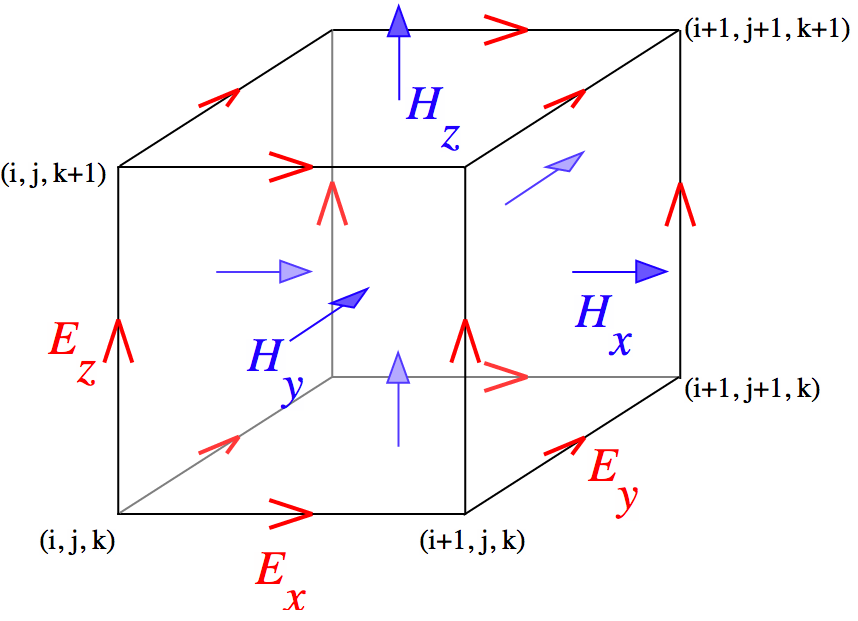
\includegraphics[width=8cm]{img/FDTDGrid.png}}
\caption{Поля в ячейке сетки FDTD. $ E $ компонента находится в середине ребер сетки, а $ H $ компонента -- в середине граней\cite{FDTDYee}.}
\label{img:FDTDGrid}
\end{figure}

Как и в любом другом разностном методе, в FDTD существует проблема неточного отображения границы тела на вычислительную сетку. Любая кривая поверхность, разделяющая соседние среды и геометрически не согласованная с сеткой, будет искажаться эффектом «лестничного приближения». Для решения данной проблемы можно использовать дополнительную сетку с большим разрешением в тех областях пространства, где расположены тела со сложной геометрической структурой.

Для того, чтобы ограничить объем сетки, в FDTD нужны особые поглощающие граничные условия, которые моделируют уход электромагнитной волны на бесконечность. Для этого используются поглощающие граничные условия Мура или Ляо, или идеально согласованные слои (Perfectly Matched Layers, PML). Условия Мура или Ляо намного проще, чем PML. Тем не менее, PML — строго говоря, являющиеся поглощающей приграничной областью, а не граничным условием как таковым — позволяют получить на порядки меньшие по величине коэффициенты отражения от границы.